\section{Case Study Design}
\label{sec:design}

In this section, we describe our: (1) rationale for selecting our studied systems and (2) data extraction process. In addition, we describe our approaches to: (3) model construction and (4) model analysis.

\subsection{Studied Systems}
\label{sec:studied}

To address our research questions, we perform a longitudinal case study on successful and rapidly evolving open source systems.
In selecting the subject systems, we identified three important criteria that needed to be satisfied:

\begin{itemize}
  \item {\bf Criterion 1: Traceability.}
    We need reliable data in order to produce healthy datasets (see Section~\ref{sec:related_bias}).
    To that end, it should be reasonably straightforward to extract from the VCS of a studied system, a series of {\em code changes}, i.e., listings of changed lines to a set of code files that developers have submitted to the VCS together.
    It should also be straightforward to connect a large proportion of those code changes to issue reports, which are stored in ITSs, and code review data, which is stored in code review databases.
    Without a traceable process, our code change properties will be unreliable, and our JIT models may be misleading.
  \item {\bf Criterion 2: Rapidly evolving.}
    In order for JIT models to yield the most benefit, our studied systems must undergo plenty of change on a continual basis.
  \item {\bf Criterion 3: Code review policy.}
    Recent studies report that code review can have an impact on post-release software quality~\cite{mcintosh2016emse,thongtanunam2015msr} and defect proneness~\cite{kononenko2015icsme}.
    To control for this, we focus our study on systems where code reviewing is a common practice.
\end{itemize}

In order to address criterion 1, we study systems that adopt the Gerrit code review tool.\footnote{\url{https://code.google.com/p/gerrit/}}
Gerrit tightly integrates with VCSs, automatically submitting commits after project-specific quality gates are passed (e.g., two reviewers vote in favour of acceptance of a change).
These Gerrit-generated commits are accompanied by a structured message, which includes references to the review record (ChangeID) and any addressed issue reports (IssueIDs).

Table~\ref{tab:cases} shows that, similar to our prior work~\cite{mcintosh2016emse, thongtanunam2016emse}, we begin with six candidate systems that adopt the Gerrit code review tool.
In order to address criterion 2, we remove {\sc ITK} from our set of candidate systems because only 3,347 changes appear in the {\sc ITK} Gerrit instance over four years.

In order to address criterion 3, we ensure that the studied systems have high rates of review coverage.
Since we find that only 55\% of {\sc VTK}, 4\% of {\sc Android}, and 14\% of {\sc LibreOffice} changes could be linked to reviews, we remove these three systems from our set of candidate systems.

Table~\ref{tab:cases} provides an overview of the two candidate systems that satisfy our selection criteria ({\sc Qt} and {\sc OpenStack}).
{\sc Qt} is a cross-platform application framework whose development is supported by the Digia corporation, however welcomes contributions from the community-at-large.\footnote{\url{http://qt.digia.com/}}
{\sc OpenStack} is an open-source software platform for cloud computing that is developed by many well-known software organizations (e.g., IBM, VMware, NEC).\footnote{\url{http://www.openstack.org/}}
Although the cleaning process is described below (see Section~\ref{sec:cleaning}), the clean {\sc Qt} dataset contains 25,150 code changes, 23,821 of which (95\%) can be linked to code reviews.
Similarly, the clean {\sc OpenStack} dataset contains 12,374 code changes, 12,041 of which (97\%) can be linked to code reviews.

\subsubsection{Gerrit Code Review Process}

\begin{figure}
  \centering
  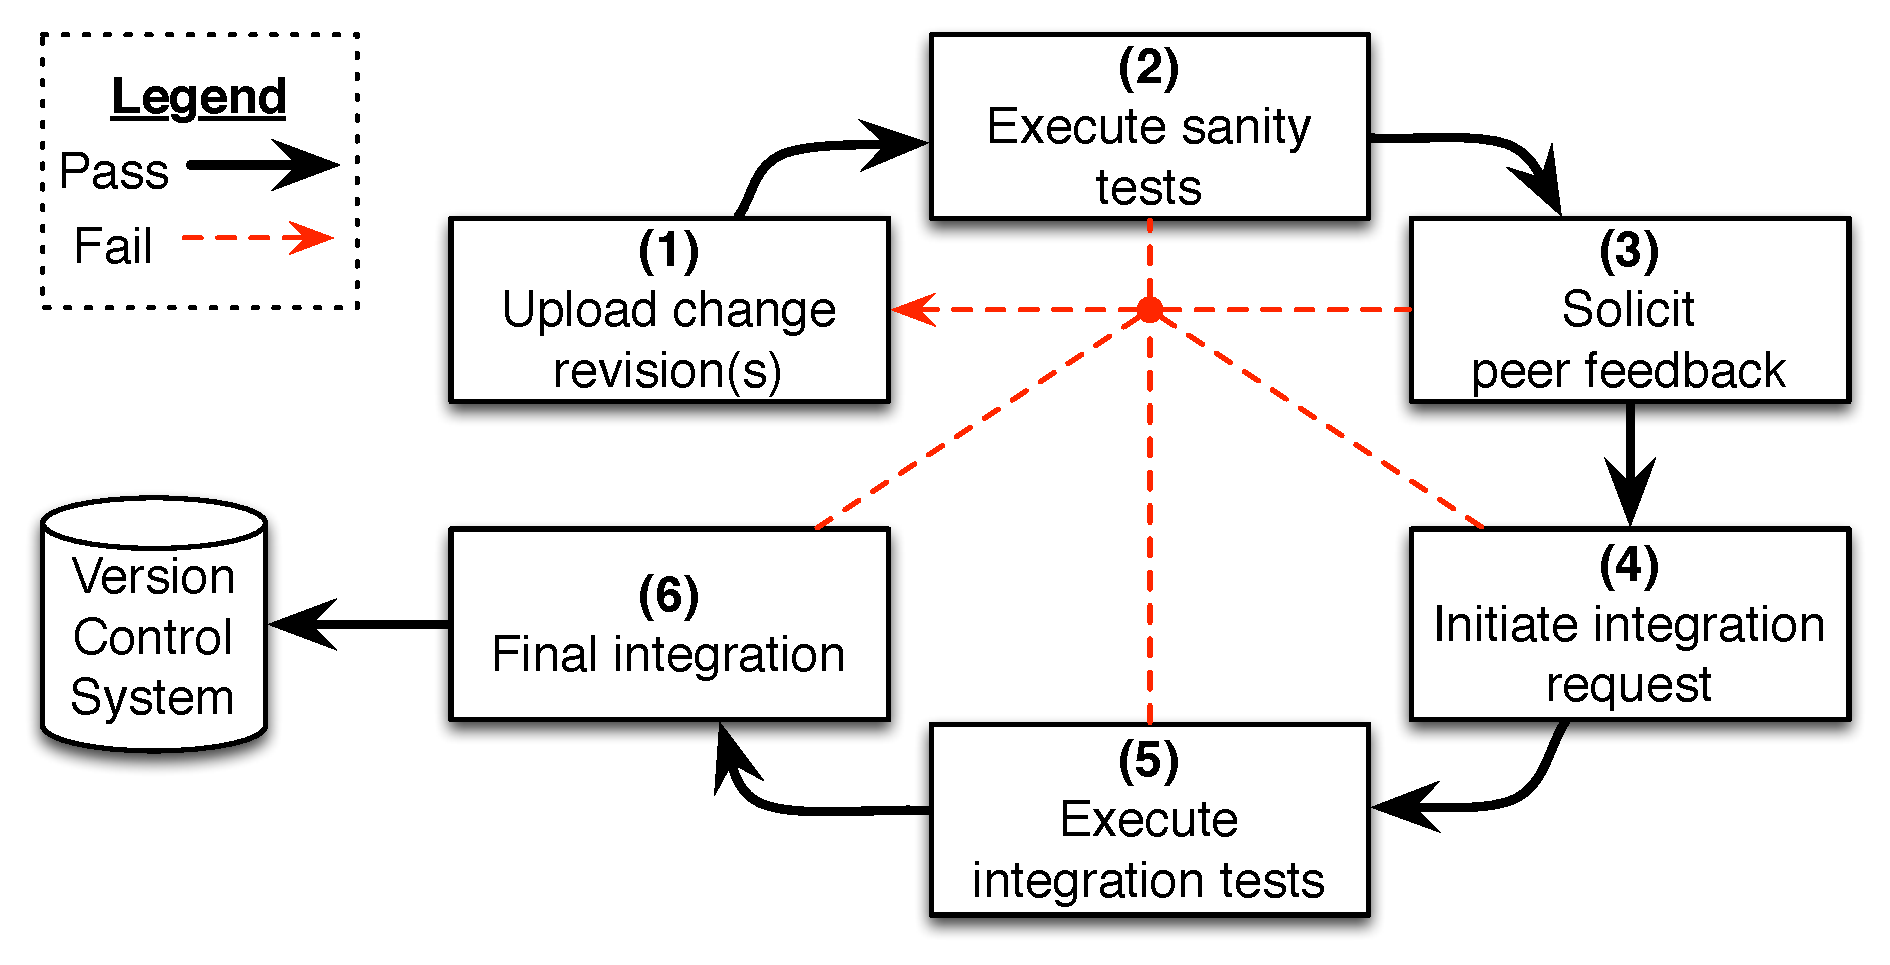
\includegraphics[width=\columnwidth]{figures/contrib_mgmt.pdf}
  \caption{An overview of the Gerrit-based code review process.}
  \label{fig:contrib_mgmt}
\end{figure}

Gerrit is a code review tool that enables a traceable code review process for {\tt git}-based software projects.
It tightly integrates with test automation and code integration tools, allowing users to codify code review and verification criteria that must be satisfied before a code change can be integrated into upstream {\tt git} repositories.

Using Gerrit, both the {\sc Qt} and {\sc OpenStack} projects implement similar workflows for managing code contributions.
Figure~\ref{fig:contrib_mgmt} provides an overview of the process, which is made up of the following steps, checks, and quality gates.

\begin{enumerate}[{\bf (1)}]
    \item {\bf Upload change revision(s).}
      An author of a code change uploads a new change or a change revision to a Gerrit instance and invites a set of reviewers to critique it by leaving comments for (a) the author to address; or (b) review participants to discuss.

    \item {\bf Execute sanity tests.}
      Before reviewers examine the submitted changes, sanity tests verify that the changes are compliant with the coding style conventions, and does not introduce obvious regression in system behaviour (e.g., code does not compile).
      If the sanity tests report issues, the change is blocked from integration until the author uploads a revision of the change that addresses the issues.
      This step provides quick feedback and avoids wasting reviewer effort on finding style or low-level coding issues that can be automatically checked.

    \item {\bf Solicit peer feedback.}
      After the submitted changes pass sanity testing, the author solicits reviewers to examine the change.
      Each reviewer is asked to provide feedback and a review score.
      In Gerrit, reviewers can provide one of five score values:
      ``+2'' indicates strong support for the change and approval for integration,
      ``+1'' indicates weak support for the change without approval for integration,
      ``0'' indicates abstention,
      ``-2'' indicates strong disagreement with the change and also blocks integration, and
      ``-1'' indicates weak disagreement with the change without blocking integration.

    \item {\bf Initiate integration request.}
      Gerrit allows teams to codify code review and verification criteria that must be satisfied before changes can be integrated into the project {\tt git} repositories.
      For example, the {\sc OpenStack} integration policy specifies that an author needs to receive at least two +2 scores.\footnote{\url{http://docs.openstack.org/infra/manual/developers.html\#project-gating}}
      After satisfying the integration criteria, the author can initiate an integration request, which queues the change for integration.

    \item {\bf Execute integration tests.}
      Code changes that are queued for integration are scanned by the integration testing system.
      The integration testing system runs a more rigourous set of tests than the sanity testing phase to ensure that changes that land in the project {\tt git} repositories are clean.
      If the integration tests report failures, the change may not be integrated until the author uploads a revision of the change that addresses the failures.

    \item {\bf Final integration.}
      Once the change passes integration testing, Gerrit automatically commits the change into the upstream (official) project {\tt git} repositories.
  \end{enumerate}

  Table~\ref{tab:cases} shows that the Gerrit-based code review processes of {\sc Qt} and {\sc OpenStack} achieve high coverage rates of 95\% and 97\%, respectively.
  On occasion, the code review process is omitted due to a rush to integrate a critical change.
  However, the vast majority of changes undergo a code review.
  Moreover, changes are rarely approved for integration by only the author.
  Only 5\% and $<$1\% of changes were self-approved in {\sc Qt} and {\sc OpenStack}, respectively.

  Table~\ref{tab:cases} also shows that more people tend to be involved in the {\sc OpenStack} review process than the {\sc Qt} one.
  The analyzed changes have a median of one reviewer in {\sc Qt} and a median of three reviewers in {\sc OpenStack}.

\begin{figure*}[t]
\centering
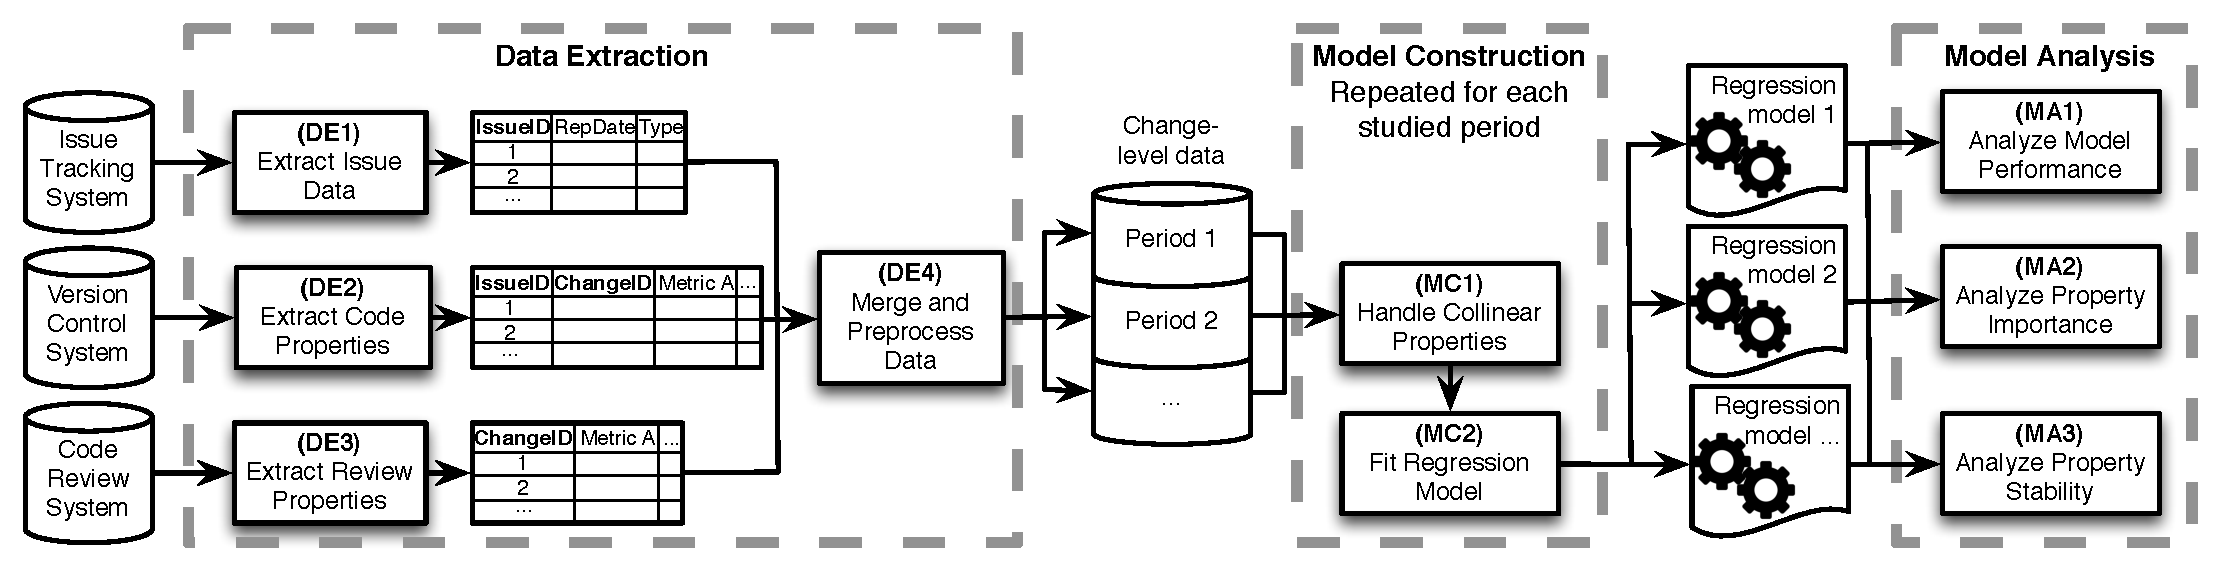
\includegraphics[width=0.98\textwidth]{figures/study_design.pdf}
\caption{An overview of the design of our case study.}
\label{fig:design}
\end{figure*}

\begin{table*}[ht!]
\centering
\caption{A taxonomy of the studied families of code and review properties.}
\label{tab:metrics}
\resizebox{\textwidth}{!}{
\begin{tabular}{c|p{2cm}|p{5.7cm}|p{8.4cm}}
\hline
& {\bf Property} & {\bf Description} & {\bf Rationale} \\
\hline
\multirow{2}{*}{\rotatebox{90}{Size}}
& Lines added & The number of lines added by a change. &  The more code that is changed, the more likely that defects \\
\cline{2-3}
& Lines deleted & The number of lines deleted by a change. & will be introduced~\cite{nagappan2006icse}.\\
\hline
\multirow{4}{*}{\rotatebox{90}{Diffusion}}
& Subsystems & The number of modified subsystems. & Scattered changes are riskier than focused ones because they \\
\cline{2-3}
& Directories & The number of modified directories. & require a broader spectrum of expertise~\cite{d2010extensive, hassan2009icse}.\\
\cline{2-3}
& Files & The number of modified files. &  \\
\cline{2-3}
& Entropy & The spread of modified lines across file. &  \\
\hline
\multirow{6}{*}{\rotatebox{90}{History}}
& Unique changes & The number of prior changes to the modified files. & More changes are likely more risky because developers will have to recall and track many previous changes~\cite{kamei2013tse}.\\
\cline{2-4}
& Developers & The number of developers who have changed the modified files in the past. & Files previously touched by more developers are likely more risky~\cite{matsumoto2010promise}. \\
\cline{2-4}
& Age & The time interval between the last and current changes. & More recently changed code is riskier than older code~\cite{graves2000tse}. \\
\hline
\multirow{11}{*}{\rotatebox{90}{Author/Rev. Experience}}
& Prior changes & The number of prior changes that an actor\smallnum{1} has participated in.\smallnum{2} & Changes that are produced by novices are likely to be more risky than changes produced by experienced developers~\cite{mockus2000bell}. \\
\cline{2-3}
& Recent changes & The number of prior changes that an actor has participated in weighted by the age of the changes (older changes are given less weight than recent ones). & \\
\cline{2-3}
& Subsystem changes & The number of prior changes to the modified subsystem(s) that an actor has participated in. & \\
\cline{2-4}
& Awareness\smallnum{3} & The proportion of the prior changes to the modified subsystem(s) that an actor has participated in. & Changes that involve developers who are aware of the prior changes in the impacted subsystems are likely to be less risky than those that do not. \\
\hline
\multirow{12}{*}{\rotatebox{90}{Review}}
& Iterations & Number of times that a change was revised prior to integration. & The quality of a change likely improves with each iteration. Hence, changes that undergo plenty of iterations prior to integration may be less risky than those that undergo few~\cite{porter1998tosem, thongtanunam2015msr}.\\
\cline{2-4}
& Reviewers & Number of reviewers who have voted on whether a change should be integrated or abandoned. & Since more reviewers will likely raise more issues so that they may be addressed prior to integration, changes with many reviewers are likely to be less risky than those with fewer reviewers~\cite{raymond}. \\
\cline{2-4}
& Comments & The number of non-automated, non-owner comments posted during the review of a change. & Changes with short discussions may not be deriving value from the review process, and hence may be more risky~\cite{mcintosh2014msr, mcintosh2016emse}.\\
\cline{2-4}
& Review window & The length of time between the creation of a review request and its final approval for integration. & Changes with shorter review windows may not have spent enough time carefully analyzing the implications of a change prior to integration, and hence may be more risky~\cite{porter1998tosem, thongtanunam2015msr}.\\
\hline
\multicolumn{4}{l}{\smallnum{1} Either the author or reviewer of a change. \smallnum{2} Either authored or reviewed. \smallnum{3} New property proposed in this paper.}
\end{tabular}
}
\end{table*}


\subsection{Data Extraction}

In order to conduct our case study, we extract data from the VCS, ITS, and code review databases of the studied systems.
Figure~\ref{fig:design} provides an overview of our data extraction approach.
Below, we describe each step in our approach.

\subsubsection*{(DE1) Extract Issue Data}
From each issue in the ITSs of the studied systems, we extract its unique identifier (IssueID), the timestamp from when the issue was reported (RepDate), and the issue type (Type, e.g., bug or enhancement).
The IssueID is used to link issues to code changes, while RepDate and Type are used to detect false positive links in our datasets.

\subsubsection*{(DE2) Extract Code Properties}
When extracting data from the VCS, we have three goals.
First, we detect whether a change is potentially fix-inducing or not using the SZZ algorithm~\cite{sliwerski2005msr}.
The SZZ algorithm identifies fix-inducing changes by:
(a) identifying defect-fixing changes,
(b) pinpointing the lines that are modified by defect-fixing changes using the {\tt diff} command,
and (c) traversing the version history to detect which change(s) introduced the modified lines using the {\tt blame} command.

Our second goal is to extract the IssueIDs and ChangeIDs that are encoded in commit messages.
The IssueIDs are used to link code changes to issue reports in the ITS, while the extracted ChangeIDs are used to link code changes to review records in the code review database.
The merging and preprocessing steps are defined in more detail under Step DE4 below.

Our third goal is to compute, for each change, four families of code change properties that have been shown to share a relationship with the likelihood of inducing fixes in past work~\cite{mockus2000bell, kim2008tse, kamei2013tse, kamei2016emse}.
We compute a broad range of code change properties that measure the change volume (Size), its dispersion across the codebase (Diffusion), the modified areas of the codebase (History), and the experience of the author (Author experience).
Table~\ref{tab:metrics} provides an overview of the studied properties.
We describe each family below.

\underline{\bf Size properties} measure the volume of code that was modified within the change.
For each change, we compute the number of {\em lines added} and {\em lines deleted}.
These properties can be directly computed by analyzing the change itself.

\newpage
\underline{\bf Diffusion properties} measure the dispersion of a change across a codebase.
For each change, we compute the number of distinct names of modified: (1) {\em subsystems} (i.e., root directories), (2) directories (i.e., full directories within the codebase), and (3) files.
To illustrate, consider the file {\tt qtbase/src/dbus/qdbuserror.cpp}.
The subsystem of this file is {\tt qtbase} and the directory is {\tt qtbase/src/dbus}.

\underline{\bf History properties} measure the past tendencies of modules that were involved with a change.
For each change, we measure history properties using the changes that have:
(a) modified the same files that are being modified by the change in question and
(b) been recorded prior to the change in question.
With this in mind, we compute the number of {\em unique changes} that have impacted the modified files in the past and the number of {\em developers} who have changed the modified files in the past.
We also compute the {\em age}, which is the average of the time intervals between the last change that was made to each modified file and the change in question.
Similar to prior studies~\cite{mockus2000bell, kamei2013tse}, we compute these history properties using all of the changes that were recorded prior to the change in question.

Files may be copied or renamed, which, if not handled carefully, may have an impact on our history properties.
In this paper, we rely on the built-in capability of {\tt git} to detect copied and renamed files.
When a copied/renamed file is detected, we include the history of the source of the copy/rename operation in the analysis of the target file.
Since {\tt git} copy/rename detection is based on heuristics, the detection results are not without limitations.
We discuss the potential impact that false positives and negatives may have on our history properties in Section~\ref{sec:cthreats}.

\begin{figure*}[t]
  \centering
  \subfloat[{\sc Qt}]{%
    \includegraphics[width=\columnwidth]{figures/filtering/qt_4.pdf}
    \label{fig:qt_filtering}
  }
  \subfloat[{\sc OpenStack}]{%
    \includegraphics[width=\columnwidth]{figures/filtering/openstack_4.pdf}
    \label{fig:openstack_filtering}
  }
  \caption{The rate of changes that are fix-inducing and the review coverage rate in the studied systems. The shaded areas are filtered out of our analysis due to large fluctuations in review coverage or drops in the rate of fix-inducing changes.}
  \label{fig:filtering}
\end{figure*}

\underline{\bf Author experience properties} estimate the expertise of the author of a change.
Similar to the history properties, author experience properties are computed using past changes.
The {\em experience} computes the number of past changes that an author has made to the codebase.
{\em Recent experience} weighs the experience value of changes by their age.
Similar to recent work~\cite{kamei2013tse}, we compute recent experience by applying $\frac{1}{1+\textit{age}}$, where {\em age} is measured in years.
{\em Subsystem experience} is the number of past changes that an author has made to the subsystems that are being modified by the change in question.
Finally, we propose author {\em awareness}---a new expertise property that measures the proportion of past changes that were made to a subsystem that the author of the change in question has authored or reviewed.
Again, Section~\ref{sec:cthreats} discusses the impact that {\tt git}'s copy/rename detection may have on our author experience measurements.

\subsubsection*{(DE3) Extract Review Properties}
When extracting data from the review databases of our studied systems, we have two goals.
First, we need to extract the ChangeIDs that are encoded in the review records.
These IDs uniquely identify a review record, and can be used to link them with code changes in the VCSs.
Next, we compute, for each review record, two families of properties that have been shown to share a relationship with the likelihood of inducing a fix~\cite{kononenko2015icsme,thongtanunam2015msr}.
We compute code review properties that measure the experience of the reviewer(s) (Reviewer experience) and characteristics of the review process (Review).
Table~\ref{tab:metrics} provides an overview of the studied review properties.
We describe each family below.

\underline{\bf Reviewer experience properties} estimate the expertise of the reviewers of a change.
Again, {\em experience} computes the number of past changes that a reviewer has reviewed,
{\em recent experience} weighs experience by age, and {\em subsystem experience} focuses on the subset of past reviews that have changed the same subsystems as the change in question.
Finally, {\em awareness} is the proportion of past changes that were made to a subsystem that the reviewer has authored or reviewed.
Again, we refer readers to Section~\ref{sec:cthreats} for a discussion of the impact that our reliance on {\tt git}'s built-in copy/rename detection may be having on our reviewer experience measurements.

\underline{\bf Review properties} estimate the investment that developers have made in the code review process.
{\em Iterations} counts the number of times that a code change was updated prior to integration.
{\em Reviewers} counts the number of developers who approved a change for integration.
{\em Comments} counts the number of reviewer comments that appear in a review record.
{\em Review window} is the length of the time interval between when a review record was opened and when the changes were approved for integration.

\begin{table}
\centering
\caption{The number of fix-inducing changes that survive each step of our filtering process.}
\label{tab:filterings}
\resizebox{\columnwidth}{!}{%
\begin{tabular}{l|p{2.5cm}|rrr|rrr}
\hline
\# & Filter & \multicolumn{3}{c|}{\sc Qt} & \multicolumn{3}{c}{\sc OpenStack} \\
   & & Total & \% & $\Delta$ & Total & \% & $\Delta$ \\
\hline
$F_0$ & No filters & 5,495 & 17\% & - & 4,423 & 16\% & - \\
$F_1$ & Code comments & 5,407 & 17\% & 88 & 4,291 & 16\% & 132 \\ 
$F_2$ & Whitespace changes  & 5,133 & 16\% & 274 & 3,814 & 14\% & 477 \\
$F_3$ & Issue report date   & 4,158 & 13\% & 975 & 3,480 & 13\% & 334 \\
$F_4$ & Issue report type & 3,242 & 10\% & 916 & 3,480 & 13\% & 0 \\
$F_{5a}$ & Too much churn & 3,190 & 10\% & 52 & 3,474 & 13\% & 6 \\
$F_{5b}$ & Too many files & 3,162 & 10\% & 28 & 3,461 & 13\% & 13 \\
$F_{5c}$ & No lines added & 3,153 & 11\% & 9 & 3,450 & 14\% & 11 \\
$F_6$ & Period & 2,891 & 11\% & 262 & 2,788 & 23\% & 662 \\
$F_7$ & Suspicious fixes & 2,172 & 9\% & 719 & 1,830 & 15\% & 958 \\
$F_8$ & Suspicious inducing changes & 2,002 & 8\% & 170 & 1,616 & 13\% & 214 \\
\hline
\end{tabular}
}
\end{table}

%F_4
%[metrics_qt5]$ awk -F, '{print $2}' all.metrics.csv.csv | sort -u | wc -l
%   31932
% awk -F, '{print $2}' qt.metrics.csv | sort -u | wc -l
%     225 -2 => 32,155
%[metrics_openstack]$ awk -F, '{print $2}' all.metrics.csv.csv | sort -u | wc -l
%   25268
% awk -F, '{print $2}' openstack.metrics.csv | sort -u | wc -l
%    1589 -2 => 26,855

\begin{comment}
# Here is the good example of white space filtering works:
-    def update_health_monitor(self, context,
-                              old_health_monitor,
-                              health_monitor,
-                              pool_id):
+    def update_pool_health_monitor(self, context,
+                                   old_health_monitor,
+                                   health_monitor,
+                                   pool_id):
\end{comment}


\subsubsection*{(DE4) Merge and Preprocess Data}
\label{sec:cleaning}

After extracting data from the VCSs, ITSs, and review databases of the studied systems, we merge them using the extracted identifiers (ChangeIDs and IssueIDs).
This merging allows us to filter our data to mitigate false positives in our datasets.
Table~\ref{tab:filterings} shows the impact of applying each filter sequentially to our sets of fix-inducing changes.

First, as suggested by Kim \ea~\cite{kim2006ase}, we ignore potential fix-inducing changes that only update code comments ($F_1$) or whitespace ($F_2$). 
Next, we filter out potential fix-inducing changes that appear after the date that the implicated defect was reported ($F_3$)~\cite{sliwerski2005msr}.
Then, we focus on only those defect-fixing changes where the issue type in the ITS is {\tt bug} ($F_4$).

After merging the datasets and cleaning the fix-inducing changes, we preprocess our dataset to remove extremities.
We ignore large commits---those that change at least 10,000 lines ($F_{5a}$) or at least 100 files ($F_{5b}$)---because these commits are likely noise that is caused by routine maintenance (e.g., copyright updates).
We also ignore changes that do not add any new lines ($F_{5c}$), since due to a limitation in the SZZ approach, only commits that introduce new lines have the potential to be flagged as fix-inducing.

In order to study whether properties of fix-inducing changes are consistent, we stratify our data into time periods.
We analyze period lengths of three and six months, since we find that at least three months are needed for our studied systems to accrue a substantial amount of data (i.e., 1,721--2,984 changes in {\sc Qt} and 831--2,094 in {\sc OpenStack}), while still yielding enough time periods to study trends (at least 18 periods in {\sc Qt} and 16 periods in {\sc OpenStack}).
Although the primary goal of our paper is not to identify the optimal period length, we discuss the threat that our choice of period lengths imposes on our conclusions in Section~\ref{sec:cthreats}.

Figure~\ref{fig:filtering} shows the results of a preliminary analysis of the rates of (a) fix-inducing changes and (b) reviewed changes in each time period ($F_6$).
We consider the rate of fix-inducing changes to counteract a limitation in the SZZ algorithm. 
The SZZ algorithm identifies defect-fixing changes, then traverses the version history to detect which change(s) had introduced the lines that were modified by the fix using the {\tt blame} command.
The SZZ algorithm needs future data to detect whether a change is fix-inducing or not.
Hence, the later the period in the analyzed data, the lower the chances that a fix has been committed to address the problems in those commits.
We do not filter out periods using a threshold value for the rate of fix-inducing changes in a period, but instead remove the latest periods where we begin to see a steady drop in the rate by analyzing Figure~\ref{fig:filtering}.

We also consider the rate of reviewed changes, since one of our criteria to select our subject systems is code review policy. However, even if the {\sc Qt} and {\sc OpenStack} projects have satisfied this criterion overall, the early periods of these projects may not.
These early periods of adoption of code review are likely turbulent as changes are being made to development processes.
To prevent the turbulent initial adoption period from impacting our reviewing measurements, we filter out periods where the review rate is low. 
Similar to the rate of fix-inducing changes, we do not select a threshold value for the rate of reviewed changes, but instead analyze Figure~\ref{fig:filtering} in search of suspicious values.

Figure~\ref{fig:qt_filtering} shows that code review coverage was sporadic in the early periods of {\sc Qt} development (periods 1--5).
Furthermore, the rate of fix-inducing changes drops dramatically in the final two development periods on record (periods 17 and 18).
Since this will introduce an additional confounding factor in our analysis, we elect to filter those periods out of our {\sc Qt} dataset.
Similarly, since Figure~\ref{fig:openstack_filtering} shows that code review coverage was extremely low for the first six development periods of {\sc OpenStack} (periods 1--6), we opt to filter those periods out of our {\sc OpenStack} dataset.

Finally, our recent work proposes a framework for evaluating the results of SZZ-generated data~\cite{costa2017tse}.
We use the framework to highlight suspicious fixes ($F_7$), i.e., changes that fix more than the upper Median Absolute Deviation (MAD) of the number of fixed issues by a change for that project.
Similarly, we use the framework to highlight suspicious fix-inducing changes as well ($F_8$), i.e., changes that induce more than the upper MAD of the number of fixes that were induced by a change for that project.

\subsection{Model Construction}
\label{sec:mc}

In this step, we use the preprocessed data to construct our JIT models.
Figure~\ref{fig:design} provides an overview of our model construction approach.
We describe each step below.

\subsubsection*{(MC1) Handle Collinear Properties}
Collinear code change properties will interfere with each other, distorting the modelled relationship between them and the likelihood of introducing defects.
Thus, we remove collinear properties prior to constructing our JIT models.

\underline{\bf Correlation analysis}:
We first check for code change properties that are highly correlated with one another using Spearman rank correlation tests ($\rho$).
We choose a rank correlation instead of other types of correlation (e.g., Pearson) because rank correlation is resilient to data that is not normally distributed.
We use a variable clustering analysis to construct a hierarchical overview of the correlation among the properties~\cite{varclus}.
For sub-hierarchies of code change properties with correlation $|\rho| > 0.7$, we select only one property from the sub-hierarchy for inclusion in our models.

\underline{\bf Redundancy analysis}:
In order to detect redundant code change properties, we fit preliminary models that explain each property using the others.
We use the $R^2$ value of these models to measure how well each property is explained by the others.
We use the implementation of this approach provided by the {\tt redun} function in the {\tt rms} R package, which iteratively drops the property that is most well-explained by the other properties until either:
(1) no model achieves an $R^2 \ge 0.9$,
or (2) removing a property would make a previously dropped property no longer explainable, i.e., its preliminary model will no longer achieve an R$^2 \ge 0.9$.

\subsubsection*{(MC2) Fit Regression Model}
We use a nonlinear variant of multiple regression modelling to fit our JIT models, which relaxes the assumption of a linear relationship between the likelihood of introducing defects and our code change properties.
This relaxed fitting technique enables a more accurate fit of the data. 
We allocate a maximum of three degrees of freedom to each property (i.e., allowing the relationship to change directions once).
Moreover, we fit our curves with restricted cubic splines, which fit smooth transitions at the points where curves change in direction (due to the curling nature of cubic curves).
Finally, as suggested by Harrell Jr. \ea~\cite{budget1, budget2}, we ensure that we do not exceed a ratio of 15 events (i.e., fix-inducing changes) per degree of freedom spent, which mitigates the risk of {\em overfitting}, i.e., producing a model that is too specialized for the training dataset to apply to others. 

The nonlinear variant of multiple regression modelling is often used in modelling of software engineering phenomena~\cite{mcintosh2016emse,morales2015saner,zhou2011icse}, especially for understanding the relationship between software development practices and software quality.
However, using other techniques may lead to different conclusions.
We discuss this threat to validity in Section~\ref{sec:ithreats}.

\subsection{Model Analysis}
\label{sec:ma}

Next, we address our research questions by analyzing our JIT models.
Figure~\ref{fig:design} provides an overview of our model analysis approach.
We describe each step below.

\subsubsection*{(MA1) Analyze Model Performance}
To assess the accuracy of our JIT models, we compute threshold-independent measures of model performance.
We avoid threshold-dependent measures like precision and recall, which depend on arbitrarily thresholds and are sensitive to imbalanced data.

The Area Under the receiver operator characteristics Curve (AUC) is a measure of a model's {\em discriminatory power}, i.e., its ability to differentiate between fix-inducing and clean changes.
AUC is computed by measuring the area under the curve that plots the true positive rate against the false positive rate, while varying the threshold that is used to determine if a change is classified as fix-inducing or not.
Values of AUC range between 0 (worst discrimination), 0.5 (random guessing), and 1 (perfect discrimination).

In addition to being a measure of discriminatory power, the Brier score is also a measure of a model's {\em calibration}, i.e., its absolute predictive accuracy.
The Brier score is computed as $\textit{Brier} = \frac{1}{N}\sum_{i=1}^{N}(y_i - \hat{y_i})^2$, where $N$ is the total number of changes; $y_i=1$ if the $i^{\textit{th}}$ change is fix-inducing, $y_i=0$ otherwise; and $\hat{y_i}$ is the probability of the $i^{\textit{th}}$ change being fix-inducing according to the JIT model under analysis.
It is important to note that low Brier scores are desirable.
Indeed, $\textit{Brier} = 0$ indicates perfect calibration, while $\textit{Brier} = 1$ indicates the worst possible calibration.

\subsubsection*{(MA2) Analyze Property Importance}
We estimate the impact that each family of code change properties has on the explanatory power of our JIT models.
In addition to each family being composed of several properties, each property has been allocated several degrees of freedom due to our nonlinear model construction approach (see Section~\ref{sec:mc}).
Each degree of freedom is represented with a model term.
Hence, to control for the effect of multiple properties (and multiple terms), we jointly test the set of model terms for each family using Wald $\chi^2$ maximum likelihood (a.k.a., ``chunk'') tests~\cite{frank}.
In order to make the Wald $\chi^2$ values of multiple models comparable, we normalize them by the total Wald $\chi^2$ score of the JIT model from which they originate.
The larger the normalized Wald $\chi^2$ score, the larger the impact that a particular family of properties has on the explanatory power of the JIT model under analysis.

\subsubsection*{(MA3) Analyze Property Stability}
To assess the stability of the importance scores for a family of code change properties $f$ over time, we compute the difference between the importance scores of $f$ in a model that is trained using time period $p$ and a future model that is trained using time period $p+x$, where $x>0$.
